\documentclass[12pt]{article}

%%%%%%%%%%%%%%%%%%%%%%%%%%%%%%%%%%%%%%%%%%%%%%%%%%%%%%%%%%%%%%%%%%%%%%%%%%%%%%%%
%                           Package preset for homework
%%%%%%%%%%%%%%%%%%%%%%%%%%%%%%%%%%%%%%%%%%%%%%%%%%%%%%%%%%%%%%%%%%%%%%%%%%%%%%%%
% Miscellaneous
\usepackage[margin=1in]{geometry}
\usepackage[utf8]{inputenc}
\usepackage{indentfirst}
\usepackage{blindtext}
\usepackage{graphicx}
\usepackage{xr-hyper}
\usepackage{hyperref}
\usepackage{enumitem}
\usepackage{color}
\usepackage{float}
% Math
\usepackage{latexsym}
\usepackage{amsfonts}
\usepackage{amssymb}
\usepackage{amsmath}
\usepackage{commath}
\usepackage{amsthm}
\usepackage{bbold}
\usepackage{bm}
% Physics
\usepackage{physics}
\usepackage{siunitx}
% Code typesetting
\usepackage{listings}
% Citation
\usepackage[authoryear]{natbib}
\usepackage{appendix}
\usepackage[capitalize]{cleveref}
% Title & name
\title{Homework}
\author{Tien Vo}
\date{\today}


%%%%%%%%%%%%%%%%%%%%%%%%%%%%%%%%%%%%%%%%%%%%%%%%%%%%%%%%%%%%%%%%%%%%%%%%%%%%%%%%
%                   User-defined commands and environments
%%%%%%%%%%%%%%%%%%%%%%%%%%%%%%%%%%%%%%%%%%%%%%%%%%%%%%%%%%%%%%%%%%%%%%%%%%%%%%%%
%%% Misc
\sisetup{load-configurations=abbreviations}
\newcommand{\due}[1]{\date{Due: #1}}
\newcommand{\hint}{\textit{Hint}}
\let\oldt\t
\renewcommand{\t}[1]{\text{#1}}

%%% Bold sets & abbrv
\newcommand{\N}{\mathbb{N}}
\newcommand{\Z}{\mathbb{Z}}
\newcommand{\R}{\mathbb{R}}
\newcommand{\Q}{\mathbb{Q}}
\let\oldP\P
\renewcommand{\P}{\mathbb{P}}
\newcommand{\LL}{\mathcal{L}}
\newcommand{\FF}{\mathcal{F}}
\newcommand{\HH}{\mathcal{H}}
\newcommand{\NN}{\mathcal{N}}
\newcommand{\ZZ}{\mathcal{Z}}
\newcommand{\RN}[1]{\textup{\uppercase\expandafter{\romannumeral#1}}}
\newcommand{\ua}{\uparrow}
\newcommand{\da}{\downarrow}

%%% Unit vectors
\newcommand{\xhat}{\vb{\hat{x}}}
\newcommand{\yhat}{\vb{\hat{y}}}
\newcommand{\zhat}{\vb{\hat{z}}}
\newcommand{\nhat}{\vb{\hat{n}}}
\newcommand{\rhat}{\vb{\hat{r}}}
\newcommand{\phihat}{\bm{\hat{\phi}}}
\newcommand{\thetahat}{\bm{\hat{\theta}}}

%%% Other math stuff
\providecommand{\units}[1]{\,\ensuremath{\mathrm{#1}}\xspace}
% Set new style for problem
\newtheoremstyle{problemstyle}  % <name>
        {10pt}                   % <space above>
        {10pt}                   % <space below>
        {\normalfont}           % <body font>
        {}                      % <indent amount}
        {\bfseries\itshape}     % <theorem head font>
        {\normalfont\bfseries:} % <punctuation after theorem head>
        {.5em}                  % <space after theorem head>
        {}                      % <theorem head spec (can be left empty, 
                                % meaning `normal')>

% Set problem environment
\theoremstyle{problemstyle}
\newtheorem{problemenv}{Problem}[section]
\newenvironment{problem}[1]{%
  \renewcommand\theproblemenv{#1}%
  \problemenv
}{\endproblemenv}
% Set lemma environment
\newenvironment{lemma}[2][Lemma]{\begin{trivlist}
\item[\hskip \labelsep {\bfseries #1}\hskip \labelsep {\bfseries #2.}]}{\end{trivlist}}
% Set solution environment
\newenvironment{solution}{
    \begin{proof}[Solution]$ $\par\nobreak\ignorespaces
}{\end{proof}}
\numberwithin{equation}{problemenv}

%%% Page format
\setlength{\parindent}{0.5cm}
\setlength{\oddsidemargin}{0in}
\setlength{\textwidth}{6.5in}
\setlength{\textheight}{8.8in}
\setlength{\topmargin}{0in}
\setlength{\headheight}{18pt}

%%% Code environments
\definecolor{dkgreen}{rgb}{0,0.6,0}
\definecolor{gray}{rgb}{0.5,0.5,0.5}
\definecolor{mauve}{rgb}{0.58,0,0.82}
\lstset{frame=tb,
  language=Python,
  aboveskip=3mm,
  belowskip=3mm,
  showstringspaces=false,
  columns=flexible,
  basicstyle={\small\ttfamily},
  numbers=none,
  numberstyle=\tiny\color{gray},
  keywordstyle=\color{blue},
  commentstyle=\color{dkgreen},
  stringstyle=\color{mauve},
  breaklines=true,
  breakatwhitespace=true,
  tabsize=4
}
\lstset{
  language=Mathematica,
  numbers=left,
  numberstyle=\tiny\color{gray},
  numbersep=5pt,
  breaklines=true,
  captionpos={t},
  frame={lines},
  rulecolor=\color{black},
  framerule=0.5pt,
  columns=flexible,
  tabsize=2
}


\title{Homework 5: Phys 5210 (Fall 2021)}

\begin{document}
\maketitle
%%%%%%%%%%%%%%%%%%%%%%%%%%%%%%%%%%%%%%%%%%%%%%%%%%%%%%%%%%%%%%%%%%%%%%%%%%%%%%%%
\begin{problem}{1}
A particle of mass $m_1$ moving with velocity $\vb{v}_1$ collides with a
particle with mass $m_2$ which is stationary, that is $\vb{v}_2=\vb{0}$. The
process can be described by splitting the motion into the center of mass motion
and relative motion. Center of mass continues to move with constant velocity
throughout the collision. Relative motion can be described by means of a vector
$\vb{r}=\vb{r}_1-\vb{r}_2$, which initially moves with the velocity
$\vb{v}=\vb{v}_1-\vb{v}_2=\vb{v}_1$. The collision process results in the
relative velocity vector turning by a certain angle $\theta$. Find the
magnitudes of the final velocities of both particles, and the angles their final
velocities form with $\vb{v}_1$.
\begin{solution}
\begin{center}
    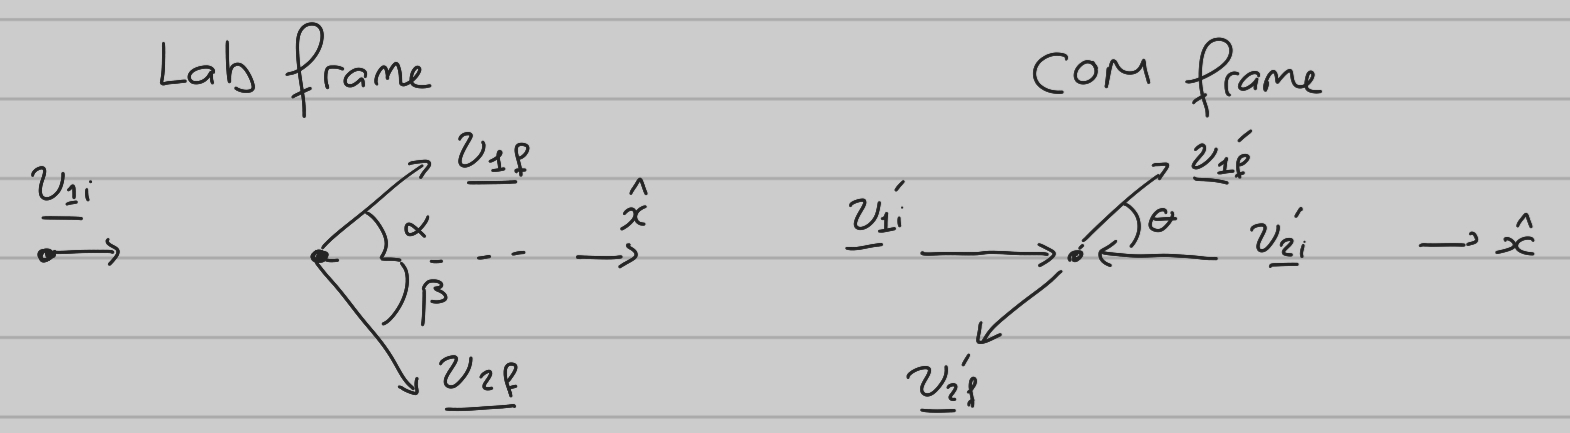
\includegraphics[width=1\textwidth]{hw5_p1.jpg} 
\end{center}
Let the un-primed coordinates be those of the lab frame, and the primed
coordinates be those of the center-of-mass (COM) frame, as denoted above. We 
know that the initial velocity of the mass $m_1$ in the lab frame is
$\vb{v}_{1i}=\vb{v}_1=v_1\xhat$ and the velocity of the COM is
$\vb{V}=m_1 /(m_1+m_2)\vb{v}_{1}=V\xhat$. By a transformation to the COM frame,
the initial velocity of the first mass is also in the $x$ direction
\begin{equation}\label{p1:v1ip}
    \vb{v}_{1i}'=\vb{v}_{1i}-\vb{V}=\frac{m_2}{m_1+m_2}v_1\xhat
\end{equation}
Now, in the COM frame, by momentum conservation, we can write
\begin{equation}
    m_1\vb{v}_{1i}'+m_2\vb{v}_{2i}'=m_1\vb{v}_{1f}'+m_2\vb{v}_{2f}'=\vb{0}
\end{equation}
This implies that
\begin{equation}\label{p1:2vs1}
    \vb{v}_{2i}'=-\frac{m_1}{m_2}\vb{v}_{1i}'
    \qquad\text{and}\qquad
    \vb{v}_{2f}'=-\frac{m_1}{m_2}\vb{v}_{1f}'
\end{equation}
By energy conservation,
\begin{alignat}{2}
    &&m_1v_{1i}'^2+m_2v_{2i}'^2
    &=m_1v_{1f}'^2+m_2v_{2f}'^2\notag\\
    &\Leftrightarrow&\qty(m_1-\frac{m_1^2}{m_2})v_{1i}'^2
    &=\qty(m_1-\frac{m_1^2}{m_2})v_{1f}'^2\notag\\
    &\Leftrightarrow&v_{1i}'&=v_{1f}'
\end{alignat}
It also follows from this that $v_{2i}'=v_{2f}'$. Then we can write the final
velocities in the lab frame from \eqref{p1:v1ip} as
\begin{equation}
    \vb{v}_{1f}=\vb{v}_{1f}'+\vb{V}=\vb{v}_{1i}'+\vb{V}
    =\qty(V+v_{1i}'\cos\theta)\xhat+v_{1i}'\sin\theta\yhat
\end{equation}
and also from \eqref{p1:2vs1}
\begin{equation}
    \vb{v}_{2f}=\vb{v}_{2f}'+\vb{V}=\vb{v}_{2i}'+\vb{V}
    =-\frac{m_1}{m_2}\vb{v}_{1f}'+\vb{V}
    =(V-\frac{m_1}{m_2}v_{1i}'\cos\theta)\xhat
    -\frac{m_1}{m_2}v_{1i}'\sin\theta\yhat
\end{equation}
Then we can calculate their magnitudes
\begin{align}
    v_{1f}&=\qty(v_{1i}'^2+V^2+2v_{1i}'V\cos\theta)^{1/2} \notag\\
          &=\qty[\frac{m_2^2}{(m_1+m_2)^2}+\frac{m_1^2}{(m_1+m_2)^2}+2\frac{m_1m_2}{(m_1+m_2)^2}\cos\theta]^{1/2}v_1\notag\\
          &=\frac{\sqrt{m_1^2+m_2^2+2m_1m_2\cos\theta}}{m_1+m_2}v_1
\end{align}
and
\begin{align}
    v_{2f}&=
    \qty(
    \frac{m_1^2}{m_2^2}v_{1i}'^2+V^2-2\frac{m_1}{m_2}v_{1i}'V\cos\theta
    )^{1/2}\notag\\
    &=\qty[\frac{m_1^2}{(m_1+m_2)^2}+\frac{m_1^2}{(m_1+m_2)^2}-2\frac{m_1^2}{(m_1+m_2)^2}\cos\theta]^{1/2}v_1\notag\\
    &=\frac{m_1}{m_1+m_2}\sqrt{2(1-\cos\theta)}v_1
\end{align}
Also, the angle $\alpha,\beta$ between $\vb{v}_{1f},\vb{v}_{2f}$ and
$\vb{v}_{1i}$ are
\begin{equation}
    \alpha=\tan^{-1}\frac{v_{1f,y}}{v_{1f,x}} 
    =\tan^{-1}\qty[\frac{\sin\theta}{\cos\theta+V/v_{1i}'}]
    =\tan^{-1}\qty[\frac{\sin\theta}{\cos\theta+m_1/m_2}]
\end{equation}
and
\begin{equation}
    \beta=\tan^{-1}\frac{v_{2f,y}}{v_{2f,x}} 
    =\tan^{-1}\qty[\frac{\sin\theta}{\cos\theta-(m_2/m_1)(V/v_{1i}')}]
    =\tan^{-1}\qty[\frac{\sin\theta}{\cos\theta-1}]
\end{equation}
\end{solution}
\end{problem}
%%%%%%%%%%%%%%%%%%%%%%%%%%%%%%%%%%%%%%%%%%%%%%%%%%%%%%%%%%%%%%%%%%%%%%%%%%%%%%%% 
%%%%%%%%%%%%%%%%%%%%%%%%%%%%%%%%%%%%%%%%%%%%%%%%%%%%%%%%%%%%%%%%%%%%%%%%%%%%%%%%
\begin{problem}{2}
A doorstop protects the wall from being slammed by a door when it is pushed
open. How far from the hinges should the doorstop be placed so that there would
be no force on the hinges as the door stops thus protecting the hinges from
breaking? Think of the door as a very thin rectangle of a uniform density
attached to the hinges at one end. To avoid thinking of the door ``falling
over'' the doorstop, think of the doorstop as a vertical pole as tall as the
door itseld, and of the door as hitting this pole at the same instant in time
along its entire length.
\begin{solution}
\begin{center}
    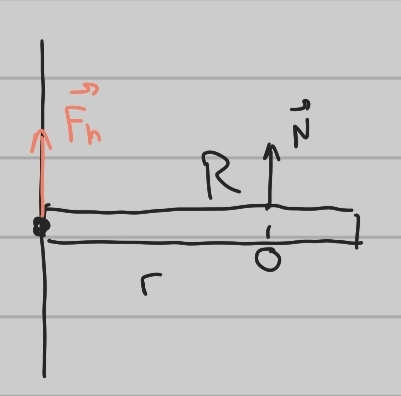
\includegraphics[width=0.4\textwidth]{hw5_p2.jpg} 
\end{center}
By Newton's 2nd Law, the total force on the door with mass $M$ (at the center 
of mass) is the sum of the force on the hinge ($\vb{F}_h$) and the normal force 
due to the doorstop $\vb{N}$
\begin{equation}\label{p2:force}
    F_h+N=Ma=\frac{MR}{2}\alpha 
\end{equation}
where we have related the angular acceleration at the center of mass of the door
($R /2$ from the hinge) to the linear acceleration $a=\alpha R /2$. Now, only
the normal force due to the doorstop causes a torque on the door
\begin{equation}\label{p2:torque}
        Nr=I\alpha 
\end{equation}
where $I=(1 /3)MR^2$ is the moment of inertia of the door (thin rectangle of
width $R$ and uniformly distributed mass) and $r$ is the
distance of the doorstop from the hinge. Substituting \eqref{p2:force} into
\eqref{p2:torque} and setting the force on the hinge $F_h=0$ results in
\begin{equation}
    \frac{MRr}{2}\alpha=I\alpha\Rightarrow\frac{MRr}{2}=\frac13MR^2
\end{equation}
Solving for $r$, we get $r=(2 /3)R$.
\end{solution}
\end{problem}
%%%%%%%%%%%%%%%%%%%%%%%%%%%%%%%%%%%%%%%%%%%%%%%%%%%%%%%%%%%%%%%%%%%%%%%%%%%%%%%%
\end{document}
